\documentclass{article}

%% Preamble
\usepackage{graphicx}
\usepackage[hidelinks]{hyperref}
\usepackage[
backend=biber,
style=apa,
]{biblatex}
\addbibresource{references.bib}
\usepackage{enumitem}
\setlength{\parskip}{6pt}
\setlength{\parindent}{0pt}
\usepackage{setspace}
\onehalfspacing
\usepackage{pgfplots}
\pgfplotsset{width=10cm,compat=1.9}
\usepackage{tikz}
\usepackage{vowel}
\usepackage{tipa}

\title{Getting Started in Overleaf}
\author{Sidney Wong}
\date{April 2025}

\begin{document}

\maketitle

\section{Getting Started}

    In \LaTeX, you will use different commands to typeset your document. Some simple commands you may be familiar with if you're used to working with word processors like Microsoft Word. Here are some example commands:
    
    \begin{verbatim}
    \documentclass{article}
    \begin{document}
        \textbf{bold}
        \textit{italic}
        \textsc{small caps}
        \texttt{typewriter}
    \end{document}
    \end{verbatim}
    \vspace{-12pt}

    And this is the output of the code chunk from above: 
    
    \begin{itemize}[nolistsep]
        \item[] \textbf{bold}
        \item[] \textit{italic}
        \item[] \textsc{small caps}
        \item[] \texttt{typewriter}
    \end{itemize}

    As your familiarity with \LaTeX\space increases, you should become more comfortable with different commands.

\newpage
\subsection{How to organise your document}

    You can organise your document into sections using the \texttt{section} commands which are equivalent to \texttt{Heading} style in Microsoft Word. You simply include the section title within the curly bracket (\texttt{\{\}}). If you do not want a number assigned to a section, you can add a star (\texttt{*}) before the curly bracket. The different section levels are:

    \begin{verbatim}
    \documentclass{article}
    \begin{document}
        \section{Heading 1}
        \subsection{Heading 2}
        \subsubsection{Heading 3}
        \paragraph{Paragraph}
        \subsubsection*{No Counter}
    \end{document}
    \end{verbatim}
    \vspace{-12pt}

    And this is the output of the code chunk from above:

    \setcounter{section}{0}
    
    \section{Heading 1}
    
    \subsection{Heading 2}
    
    \subsubsection{Heading 3}

    \paragraph{Paragraph}

    \subsubsection*{No Counter}
    
    You can use the section command to signpost your document. You can also produce a table of contents based on the section command.
    
    \setcounter{section}{2}

\newpage
\subsection{How to create a list}

    Creating a bulleted or numbered list is relatively straightforward. Here's an example of a bulleted list:
    
    \begin{verbatim}
    \documentclass{article}
    \begin{document}
        \begin{itemize}[nolistsep]
            \item Item 1
            \item Item 2
            \item Item 3
        \end{itemize}
    \end{document}
    \end{verbatim}
    \vspace{-12pt}
    
    And this is the output of the code chunk from above:

    \vspace{12pt}
    \begin{itemize}[nolistsep]
        \item Item 1
        \item Item 2
        \item Item 3
    \end{itemize}

\newpage
\subsection{How to create a table}

    Creating a table is similarly straightforward. Here's an example of a table:

    \begin{verbatim}
    \documentclass{article}
    \begin{document}
        \begin{table}[h]
            \centering
            \begin{tabular}{lc}
                \hline
                 \textbf{Category} & $n$ \\
                 \hline
                 Item & 1 \\
                 Item & 2 \\
                 Item & 3 \\
                 \hline
            \end{tabular}
            \caption{Example table}
        \end{table}
    \end{document}
    \end{verbatim}
    \vspace{-12pt}

    And this is the output of the code chunk from above:

    \vspace{12pt}
    \begin{table}[h]
        \centering
        \begin{tabular}{lc}
            \hline
             \textbf{Category} & $n$ \\
             \hline
             Item & 1 \\
             Item & 2 \\
             Item & 3 \\
             \hline
        \end{tabular}
        \caption{Example table}
    \end{table}

\newpage
\subsection{How to add a figure}

    You can also insert \texttt{.png} or \texttt{.jpeg} figures to your document. These figures can either be saved locally in the working environment or online called by its URL. Here's an example of a figure from the Noun Project when I searched for \textit{linguistics}:

    \begin{verbatim}
    \documentclass{article}
    \begin{document}
        \begin{figure}[h]
            \centering
            
\includegraphics[width=0.5\linewidth]{figures/linguistics.png}
            \caption{Linguistics}
        \end{figure}
    \end{document}
    \end{verbatim}
    \vspace{-12pt}

    And this is the output of the code chunk from above:

    \vspace{12pt}
    \begin{figure}[h]
        \centering
        
\includegraphics[width=0.5\linewidth]{figures/linguistics.png}
        \caption{Linguistics}
    \end{figure}

\newpage
\subsection{How to reference}

    One of the main benefits for using \LaTeX\space is its ability to support different citation methods. With the \texttt{biblatex} package (one of the two main citation packages, the other one being \texttt{natbib}), you can easily include in text citations in your document. 
    
    You can modify the bibliography style and the \texttt{printbibliography} command to produce a bibliography/reference section as shown in this document. You will first need to create a \texttt{.bib} file, you can use the following commands to produce in text citations:
    
    \begin{itemize}[nolistsep]
        \item \texttt{cite}: \cite{dunn_stability_2022}
        \item \texttt{textcite}: \textcite{dunn_stability_2022}
        \item \texttt{parencite}: \parencite{dunn_stability_2022}
    \end{itemize}

    You can also print the full citation using the \texttt{fullcite} command:

    \hspace{12pt}\fullcite{dunn_stability_2022}

    Of course, you're not expected to create a \texttt{.bib} file from scratch. You can integrate your Zotero account with your Overleaf project by uploading a public library to your project. You should expect to see the following window when you upload the file.
    
    \begin{figure}[h]
        \centering
        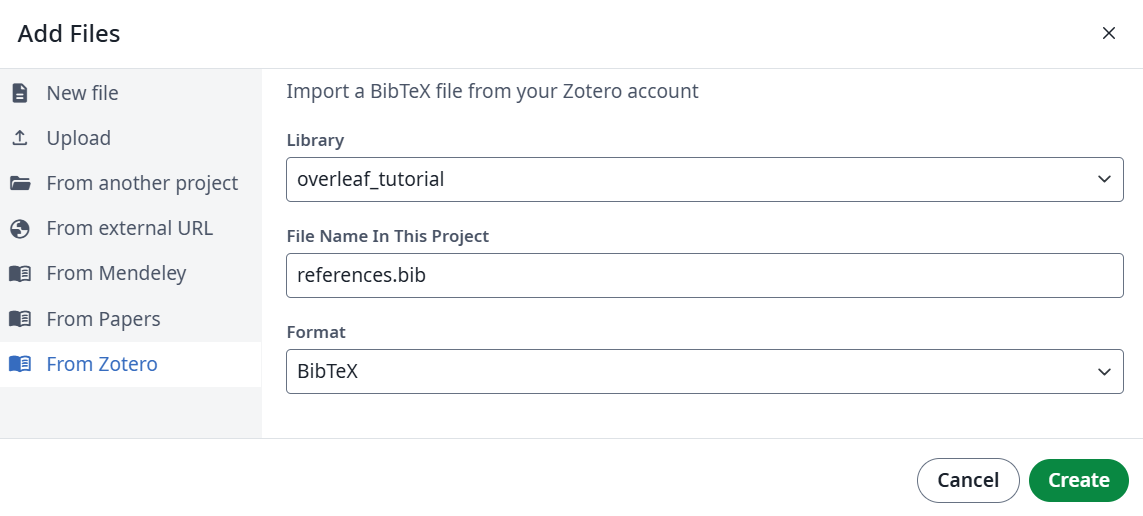
\includegraphics[width=\linewidth]{figures/zotero.png}
        \caption{Add Files}
    \end{figure}
 
\newpage
\section{Extra for Experts}

    You can also create graphs in \LaTeX. This is a fairly complex example of a graph from \textcite{trudgill_sex_1972}, so don't worry if you don't understand what is happening in the code.

    \vspace{12pt}
    \begin{figure}[ht]
    \caption{\cite{trudgill_sex_1972}}
    \centering
    \vspace{6pt}
        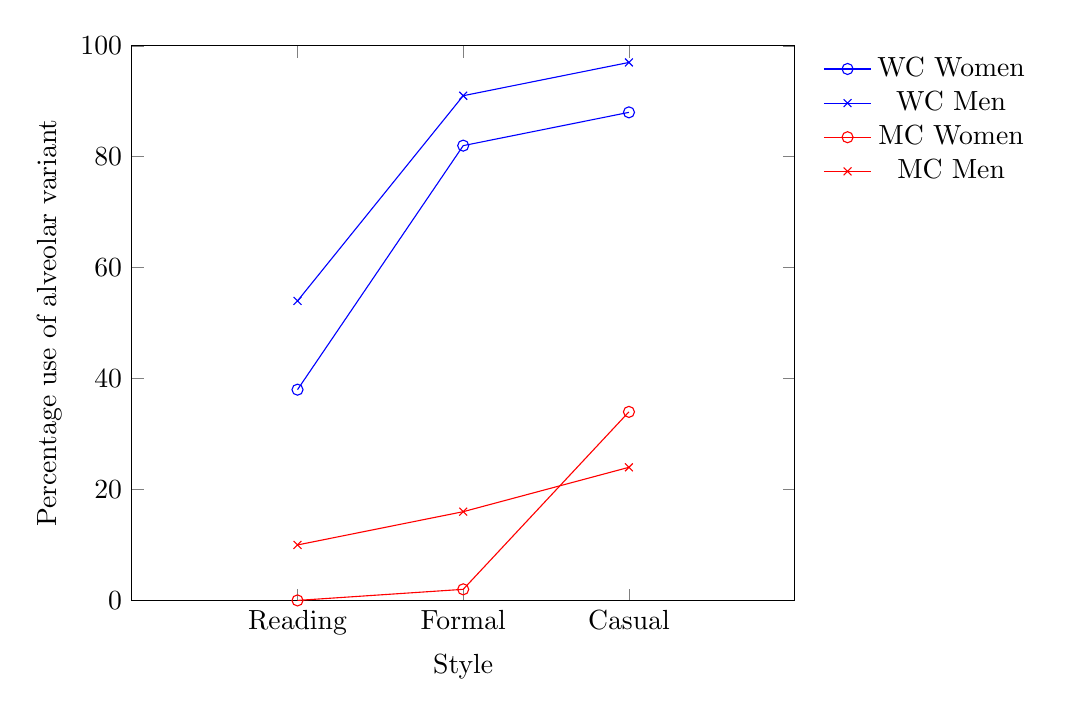
\begin{tikzpicture}
            \begin{axis}[
                xlabel={Style},
                ylabel={Percentage use of alveolar variant},
                xmin=0, xmax=4,
                ymin=-0, ymax=100,
                xtick={0,1,2,3},
                ytick={0,20,40,60,80,100},
                legend pos=outer north east,
                legend style={draw=none},
                xticklabels={Reading, Formal, Casual},xtick={1,2,3}],
                ymajorgrids=true,
                grid style=dashed,
            ]
            \addplot[color=blue,mark=o,]
                coordinates {(1,38)(2,82)(3,88)};
            \addplot[color=blue,mark=x,]
                coordinates {(1,54)(2,91)(3,97)};
            \addplot[color=red,mark=o,]
                coordinates {(1,0)(2,2)(3,34)};
            \addplot[color=red,mark=x,]
                coordinates {(1,10)(2,16)(3,24)};
                \legend{WC Women, 
                WC Men,
                MC Women,
                MC Men}
            \end{axis}
        \end{tikzpicture}
    \end{figure}

    You can check out the code on the next page:

    \newpage
    \begin{verbatim}
    \documentclass{article}
    \begin{document}
    \usepackage{pgfplots}
    \pgfplotsset{width=10cm,compat=1.9}
    \usepackage{tikz}
    \begin{figure}[ht]
        \caption{\citet{trudgill_sex_1972}}
        \centering
        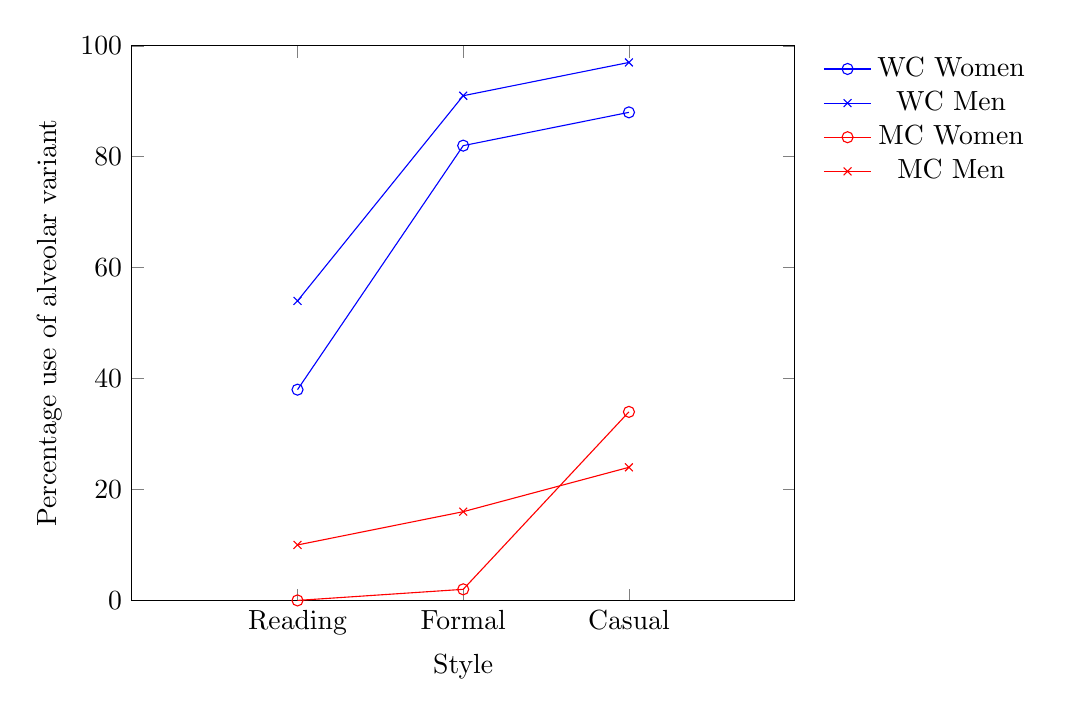
\begin{tikzpicture}
            \begin{axis}[
                xlabel={Style},
                ylabel={Percentage use of alveolar variant},
                xmin=0, xmax=4,
                ymin=-0, ymax=100,
                xtick={0,1,2,3},
                ytick={0,20,40,60,80,100},
                legend pos=outer north east,
                legend style={draw=none},
                xticklabels={Reading, Formal, Casual},xtick={1,2,3}],
                ymajorgrids=true,
                grid style=dashed,]
            \addplot[color=blue,mark=o,]
                coordinates {(1,38)(2,82)(3,88)};
            \addplot[color=blue,mark=x,]
                coordinates {(1,54)(2,91)(3,97)};
            \addplot[color=red,mark=o,]
                coordinates {(1,0)(2,2)(3,34)};
            \addplot[color=red,mark=x,]
                coordinates {(1,10)(2,16)(3,24)};
                \legend{WC Women, 
                WC Men,
                MC Women,
                MC Men}
            \end{axis}
        \end{tikzpicture}
    \end{figure}
    \end{document}
    \end{verbatim}

    And here's another example on how to produce a vowel space Typical vowel space of New Zealand English Speaker adapted from \textcite{gordon_new_2008} using the \texttt{vowel} and \texttt{tipa} packages.
    
    \begin{figure}[ht]
        \Large
        \centering
        \caption{Typical vowel space of New Zealand English Speaker.}
        \vspace{6pt}
        \begin{vowel}[ipanew]
            \putcvowel{\ae}{3}
            \putcvowel{a\textlengthmark}{4}
            \putcvowel{e}{2}
            \putcvowel{\textturna}{15}
            \putcvowel{\textschwa}{10}
            \putcvowel{\textbaru\textlengthmark}{14}
        \end{vowel}
    \end{figure}

    You can check out the code below:
    
    \begin{verbatim}
    \documentclass{article}
    \begin{document}
    \begin{figure}[ht]
        \usepackage{vowel}
        \usepackage{tipa}
        \Large
        \centering
        \caption{Typical vowel space of New Zealand English Speaker.}
        \vspace{6pt}
        \begin{vowel}[ipanew]
            \putcvowel{\ae}{3}
            \putcvowel{a\textlengthmark}{4}
            \putcvowel{e}{2}
            \putcvowel{\textturna}{15}
            \putcvowel{\textschwa}{10}
            \putcvowel{\textbaru\textlengthmark}{14}
        \end{vowel}
    \end{figure}
    \end{document}
    \end{verbatim}

\section{Summary}

    This is just a quick overview of \LaTeX\space environment in Overleaf. Once you get started, you're on your way to being a typesetting genius. If you have any questions, please feel free to get in touch at: \href{sidney.wong@pg.canterbury.ac.nz}{sidney.wong@pg.canterbury.ac.nz}.

\printbibliography

\end{document}
